\chapter{Velvet Fork Implementation}
We implement ... motivation TODO ...

Since Bitcoin Cash blocks don't contain the interlink we have to utilize a User-Activated Velvet Fork. To this end, we need to make sure that a transaction is included in every single block containing its implied interlink. We do this by implementing a service which for every new block, calculates the expected interlink of the upcoming block and sends a transaction including this interlink in hopes that it will be included in the upcoming block. If this is indeed achieved then that block will indeed contain its valid interlink. We henceforth call the service which does this an \emph{interlinker}.

\section{Interlink encoding}
Including the whole interlink inside the transaction would make the transaction really big. Assuming a naive encoding of the interlink v, where each 256-bit block hash from level $0$ up to $\infty$ is concatenated, on the Bitcoin Cash testnet at the time of writing just the interlink would be 704 bytes. In Bitcoin Cash the fee of the transaction is proportional to the transaction size, and since we're going to be sending a transaction for every block (which is mined approximately every 10 minutes), it is important that we keep this cost down. 

bitcoin cash levels TODO
bitcoin cash uses sha256 TODO explain size estimate of naive method

In order to save space, we only include a commitment to the interlink in our transactions. Specifically, we take the Merkle Tree root of the Merkle Tree with leafs the block hashes starting from level $0$ up to $\infty$. This way, our interlink encoding is constant size and we can easily provide compact proofs for any of the levels. TODO give numbers

bitcoin cash (testnet) levels merkle tree TODO
bitcoin cash (testnet) logarithmic scale histogram of block levels TODO
bitcoin cash blocks incl merkle tree for tx incl merkle tree for interlink incl coloring for some some interlink lvl TODO

example chain with super blocks and actual merkle tree proof for interlink and tree with examples (mock 16-bit values) TODO

\section{Discoverability}
We've talked about how just including the interlink somewhere on a block is what really matters but it is crucial that we make this information easy to discover. We achieve this in two ways. First, we include the interlink commitment inside a special \code{OP\_RETURN} output. Such outputs are already being used for storing arbitrary data in blocks~\cite{arbitrary-data} therefore we adopt this method for storing our interlinks. Second, we aim to make this interlink discoverable for lite nodes, so we don't require our users to download a whole block in order to look into it. We achieve this by utilizing a method called \emph{SPV tagged outputs}~\cite{spv-tagged}.

SPV tagged outputs are outputs that are tagged so that they can be discovered by SPV nodes who add the ``tag'' to the filter. Specifically, we form outputs of the form \code{OP\_RETURN baba deadbeef}, where \code{baba} is our tag and \code{deadbeef} is our payload (in our case, the interlink commitment). A bloom filter for \code{baba} will then match this output and subsequently the transaction that contains it and this is how our specialized SPV nodes can discover our outputs. The full nodes forwarding the velvet transactions to the SPV nodes don't have any knowledge of what a velvet fork even is, let alone that they are forwarding its transactions.

The tag we use for our transactions is \code{696e7465726c696e6b}, which is the ASCII encoding of \code{interlink}. An example of such a real-world velvet transaction created by our deployed interlinker on the Bitcoin Cash testnet can be seen on Figure~\ref{fig:actual-velvet-tx}.

\begin{figure}
  \centering
  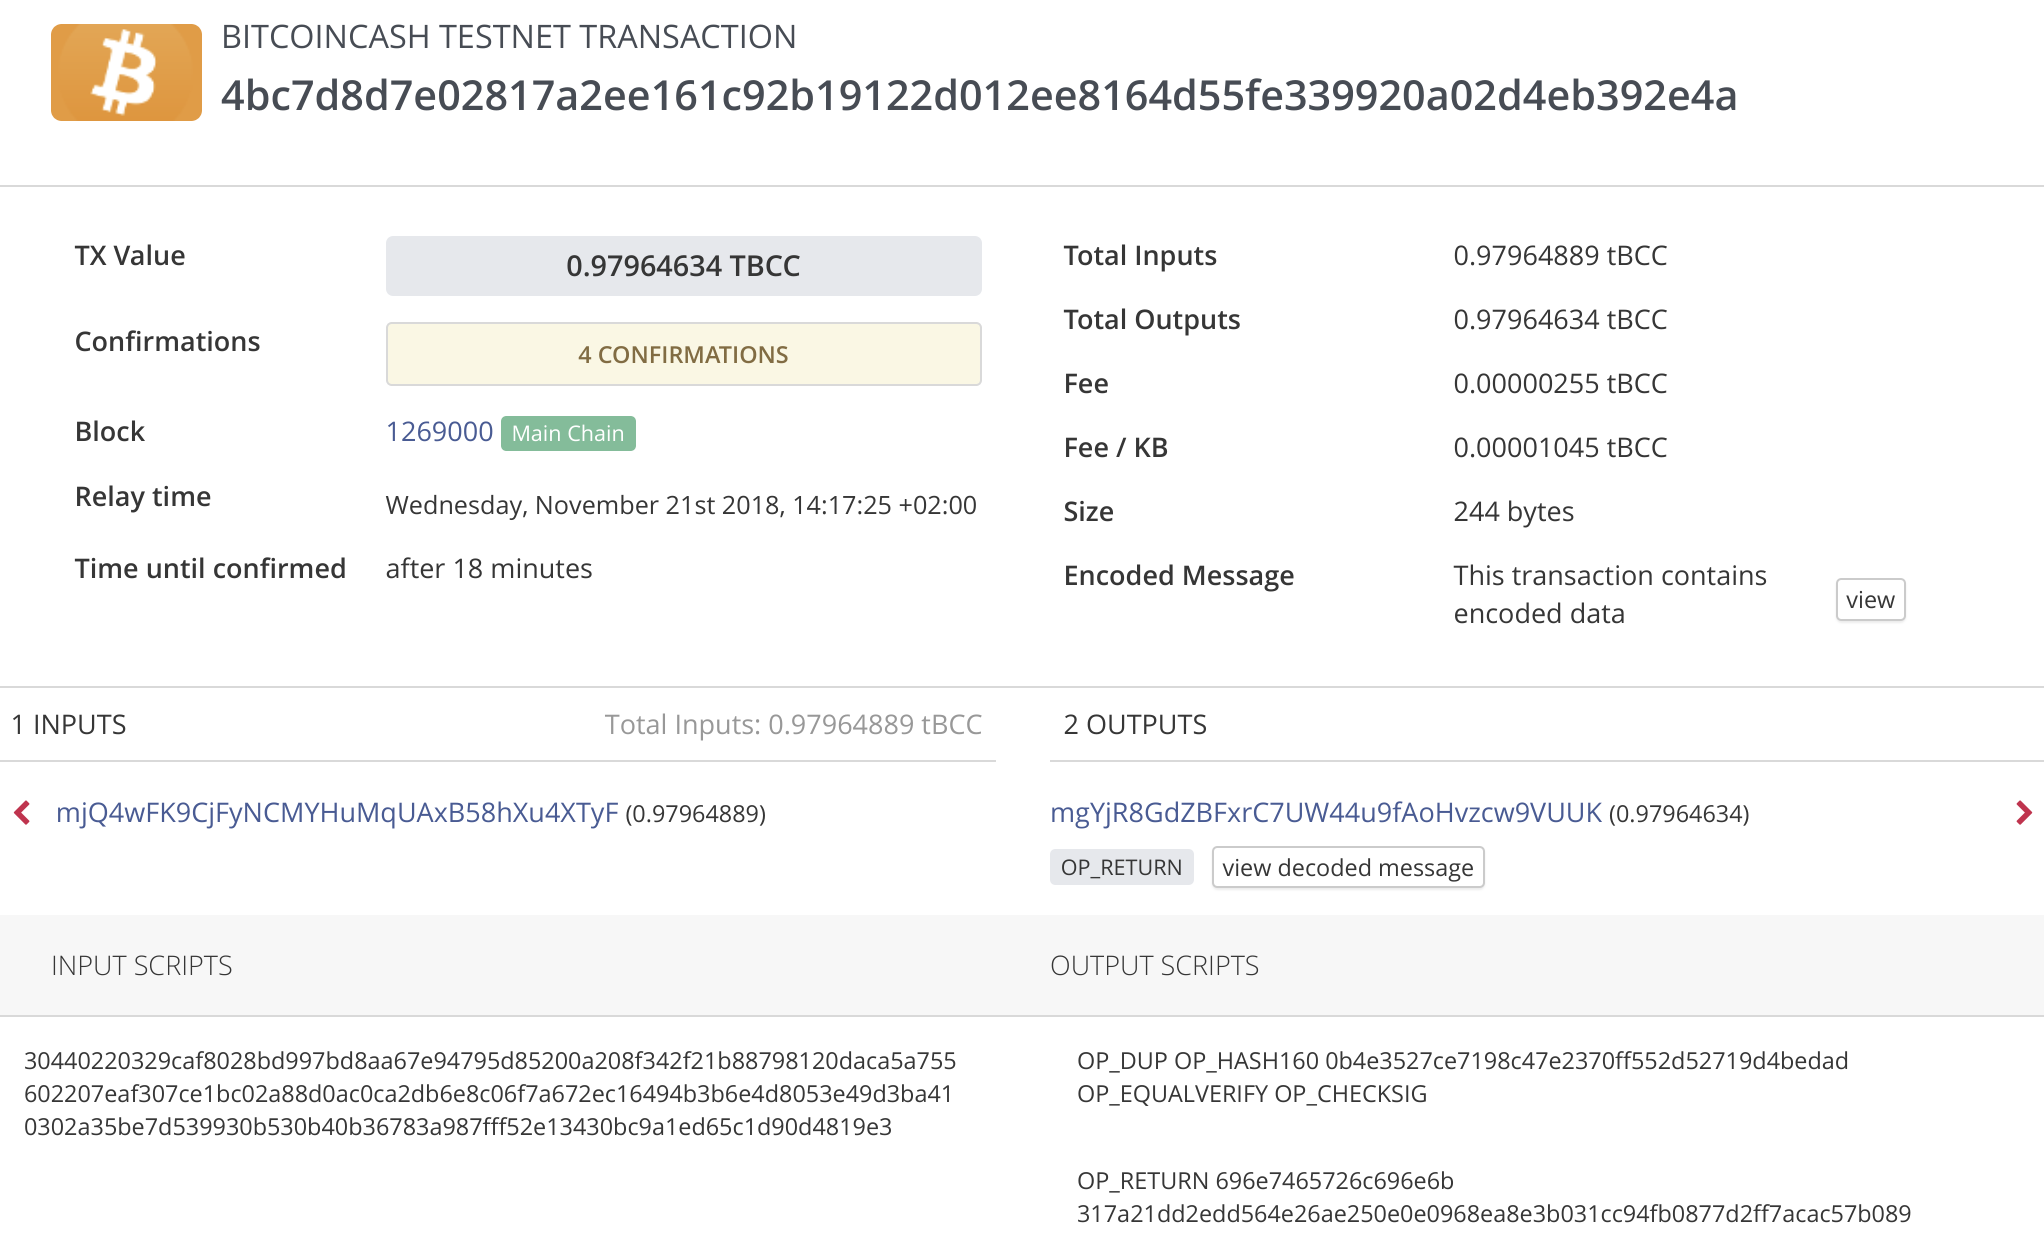
\includegraphics[width=0.9\columnwidth,keepaspectratio]{figures/actual-velvet-tx.png}
  \caption{An actual velvet fork transaction.}
  \label{fig:actual-velvet-tx}
\end{figure}

\section{Fault Tolerance}
It is important to note that the interlinker works on a best-effort basis. Due to the nature of Velvet Forks though, no failure is fatal. The types of failures are as follows:

\begin{itemize}
  \item \textbf{Crash failure}: The interlinker crashes or halts.
  \item \textbf{Omission failure}: The interlinker fails to push a transaction upon seeing a new block.
  \item \textbf{Timing failure}: The interlinker pushes a transaction which fails to be included in the upcoming block.
  \item \textbf{Response failure}: The interlinker pushes a transaction with an invalid interlink.
  \item \textbf{Arbitrary failure}: The interlinker pushes a transaction before a new block is seen or pushes a duplicate for a specific upcoming block twice.
\end{itemize}

We will study how these failures can be mitigated in the next section.

\section{Viability}
Making the operation of the interlinker affordable is key in order to allow many parties to run it. We will estimate the cost of operation now.

Our transaction size ($\sf txBytes$) is constant at exactly 244 bytes. The median Bitcoin Cash fee per byte ($\sf feePerByte$) at the time of writing (November 2018) is 1 satoshi. Multiplied by our transaction size this gives us a transaction fee ($\sf txFee = txBytes * feePerByte$) of 244 satoshis.

\begin{table}
  \centering
  \begin{tabular}{|c|c|c|}
    \hline
    Cost per & Formula & Current estimation \\
    \hline
    Day & $\sf txFee * 10 * 24$ & 0.13€ \\
    Month & $\sf perDay * 30$ & 3.9€ \\
    Year & $\sf perMonth * 12$ & 46.8€ \\
    \hline
  \end{tabular}
\end{table}

We provide two implementations of an interlinker. Since the writing of this thesis, both interlinkers run in production on the Bitcoin Cash testnet chain. We'll now look at the pros and cons of each.

TODO during the period xxx to yyy we observed the following experimental data:
x\% valid transactions TODO
overhead TODO
interlinker size TODO
levels TODO

\section{Bitcoin-ABC}
Our first implementation is built on top of Bitcoin-ABC. Bitcoin-ABC is the reference implementation for Bitcoin Cash in C++. It is a fork of the original Bitcoin codebase (now Bitcoin Core), and it was the first ever implementation to support Bitcoin Cash. It has a very active community of developers and users. Due to its heritage from Bitcoin Core the code is very well written and tested, and any new feature for the Bitcoin Cash chain appears on Bitcoin-ABC first.

We run Bitcoin-ABC as a full node and interface with it using JSON-RPC. The interlinker is a Python module which knows (a) the location and credentials to connect with the full node and (b) the velvet fork genesis block id (TODO major explain).

TODO which genesis we picked

After the interlinker makes sure the full node is fully synced it starts waiting for new blocks. As described above we need our interlinker to get notified whenever there's a new block so that it can send a transaction with the new interlink for inclusion in the upcoming block. There's two options to get notified for new blocks from a full node.

The first option is to utilize the ZeroMQ~\cite{zmq} functionality of Bitcoin-ABC. If compiled with the appropriate flags, Bitcoin-ABC can create a ZeroMQ channel where it will send notifications for new blocks and transactions. While the method seems very modern, it has some pitfalls. The main pitfall is race conditions: it is possible that the node pushes out a ZeroMQ notification about a block, however that block has not finished saving in the node's database, causing an immediate \code{getblock} request on the block to fail. Also, the ZeroMQ functionality is not enabled by default: one needs to compile the node with specific flags. While both issues are not fatal, in order to keep the interlinker as compatible with existing nodes as possible and to avoid workarounds we decided against using this functionality.

What we ended up using is busy polling through JSON-RPC with the \code{getbestblockhash} method. Every 5 seconds the interlinker will check the best block hash and if it doesn't match the one previously given then this means that there's been a new block. The interval can be configured should one desire not to cause much strain to their system.

In case there's a new block, the interlinker will promptly compute the correct interlink for it, by updating the interlink with all the intermediate blocks from the velvet fork genesis up to and including the new block. It will then compute the Merkle Tree root and include it in an SPV tagged output. It will then wrap the output inside a change transaction and send it to the network.

It is important to note here that in order to send the transactions, the interlinker has to spend funds (because of tx fees TODO). However, we haven't talked about the interlinker controlling a wallet or private keys which would make it seem like there is no way to fund the transactions. Because of how the JSON-RPC methods work we don't need to specify a private key or wallet external to the full node and we can let the full node create and pay for our transactions using its default wallet. Thus the way to fund the interlinker is to fund the default wallet of the full node.

show transaction TODO
show transaction chain TODO
velvet txs in in correct block confirmed later TODO

code for interlink calculation TODO
code snippets TODO

\section{bcash}
The second implementation is build on top of the bcash JavaScript library. bcash implements a full node and wallet functionality exclusively in JavaScript without being based on the Bitcoin C++ codebase as did most previous solutions. A major advantage of bcash is that it implements an SPV node too, which is very useful since the interlinker only needs the block ids of the chain but doesn't care about the block contents, so requiring a full node to run it would be a waste of space and bandwidth.
